% Options for packages loaded elsewhere
\PassOptionsToPackage{unicode}{hyperref}
\PassOptionsToPackage{hyphens}{url}
%
\documentclass[
]{book}
\usepackage{amsmath,amssymb}
\usepackage{lmodern}
\usepackage{iftex}
\ifPDFTeX
  \usepackage[T1]{fontenc}
  \usepackage[utf8]{inputenc}
  \usepackage{textcomp} % provide euro and other symbols
\else % if luatex or xetex
  \usepackage{unicode-math}
  \defaultfontfeatures{Scale=MatchLowercase}
  \defaultfontfeatures[\rmfamily]{Ligatures=TeX,Scale=1}
\fi
% Use upquote if available, for straight quotes in verbatim environments
\IfFileExists{upquote.sty}{\usepackage{upquote}}{}
\IfFileExists{microtype.sty}{% use microtype if available
  \usepackage[]{microtype}
  \UseMicrotypeSet[protrusion]{basicmath} % disable protrusion for tt fonts
}{}
\makeatletter
\@ifundefined{KOMAClassName}{% if non-KOMA class
  \IfFileExists{parskip.sty}{%
    \usepackage{parskip}
  }{% else
    \setlength{\parindent}{0pt}
    \setlength{\parskip}{6pt plus 2pt minus 1pt}}
}{% if KOMA class
  \KOMAoptions{parskip=half}}
\makeatother
\usepackage{xcolor}
\usepackage{color}
\usepackage{fancyvrb}
\newcommand{\VerbBar}{|}
\newcommand{\VERB}{\Verb[commandchars=\\\{\}]}
\DefineVerbatimEnvironment{Highlighting}{Verbatim}{commandchars=\\\{\}}
% Add ',fontsize=\small' for more characters per line
\usepackage{framed}
\definecolor{shadecolor}{RGB}{248,248,248}
\newenvironment{Shaded}{\begin{snugshade}}{\end{snugshade}}
\newcommand{\AlertTok}[1]{\textcolor[rgb]{0.94,0.16,0.16}{#1}}
\newcommand{\AnnotationTok}[1]{\textcolor[rgb]{0.56,0.35,0.01}{\textbf{\textit{#1}}}}
\newcommand{\AttributeTok}[1]{\textcolor[rgb]{0.77,0.63,0.00}{#1}}
\newcommand{\BaseNTok}[1]{\textcolor[rgb]{0.00,0.00,0.81}{#1}}
\newcommand{\BuiltInTok}[1]{#1}
\newcommand{\CharTok}[1]{\textcolor[rgb]{0.31,0.60,0.02}{#1}}
\newcommand{\CommentTok}[1]{\textcolor[rgb]{0.56,0.35,0.01}{\textit{#1}}}
\newcommand{\CommentVarTok}[1]{\textcolor[rgb]{0.56,0.35,0.01}{\textbf{\textit{#1}}}}
\newcommand{\ConstantTok}[1]{\textcolor[rgb]{0.00,0.00,0.00}{#1}}
\newcommand{\ControlFlowTok}[1]{\textcolor[rgb]{0.13,0.29,0.53}{\textbf{#1}}}
\newcommand{\DataTypeTok}[1]{\textcolor[rgb]{0.13,0.29,0.53}{#1}}
\newcommand{\DecValTok}[1]{\textcolor[rgb]{0.00,0.00,0.81}{#1}}
\newcommand{\DocumentationTok}[1]{\textcolor[rgb]{0.56,0.35,0.01}{\textbf{\textit{#1}}}}
\newcommand{\ErrorTok}[1]{\textcolor[rgb]{0.64,0.00,0.00}{\textbf{#1}}}
\newcommand{\ExtensionTok}[1]{#1}
\newcommand{\FloatTok}[1]{\textcolor[rgb]{0.00,0.00,0.81}{#1}}
\newcommand{\FunctionTok}[1]{\textcolor[rgb]{0.00,0.00,0.00}{#1}}
\newcommand{\ImportTok}[1]{#1}
\newcommand{\InformationTok}[1]{\textcolor[rgb]{0.56,0.35,0.01}{\textbf{\textit{#1}}}}
\newcommand{\KeywordTok}[1]{\textcolor[rgb]{0.13,0.29,0.53}{\textbf{#1}}}
\newcommand{\NormalTok}[1]{#1}
\newcommand{\OperatorTok}[1]{\textcolor[rgb]{0.81,0.36,0.00}{\textbf{#1}}}
\newcommand{\OtherTok}[1]{\textcolor[rgb]{0.56,0.35,0.01}{#1}}
\newcommand{\PreprocessorTok}[1]{\textcolor[rgb]{0.56,0.35,0.01}{\textit{#1}}}
\newcommand{\RegionMarkerTok}[1]{#1}
\newcommand{\SpecialCharTok}[1]{\textcolor[rgb]{0.00,0.00,0.00}{#1}}
\newcommand{\SpecialStringTok}[1]{\textcolor[rgb]{0.31,0.60,0.02}{#1}}
\newcommand{\StringTok}[1]{\textcolor[rgb]{0.31,0.60,0.02}{#1}}
\newcommand{\VariableTok}[1]{\textcolor[rgb]{0.00,0.00,0.00}{#1}}
\newcommand{\VerbatimStringTok}[1]{\textcolor[rgb]{0.31,0.60,0.02}{#1}}
\newcommand{\WarningTok}[1]{\textcolor[rgb]{0.56,0.35,0.01}{\textbf{\textit{#1}}}}
\usepackage{longtable,booktabs,array}
\usepackage{calc} % for calculating minipage widths
% Correct order of tables after \paragraph or \subparagraph
\usepackage{etoolbox}
\makeatletter
\patchcmd\longtable{\par}{\if@noskipsec\mbox{}\fi\par}{}{}
\makeatother
% Allow footnotes in longtable head/foot
\IfFileExists{footnotehyper.sty}{\usepackage{footnotehyper}}{\usepackage{footnote}}
\makesavenoteenv{longtable}
\usepackage{graphicx}
\makeatletter
\def\maxwidth{\ifdim\Gin@nat@width>\linewidth\linewidth\else\Gin@nat@width\fi}
\def\maxheight{\ifdim\Gin@nat@height>\textheight\textheight\else\Gin@nat@height\fi}
\makeatother
% Scale images if necessary, so that they will not overflow the page
% margins by default, and it is still possible to overwrite the defaults
% using explicit options in \includegraphics[width, height, ...]{}
\setkeys{Gin}{width=\maxwidth,height=\maxheight,keepaspectratio}
% Set default figure placement to htbp
\makeatletter
\def\fps@figure{htbp}
\makeatother
\setlength{\emergencystretch}{3em} % prevent overfull lines
\providecommand{\tightlist}{%
  \setlength{\itemsep}{0pt}\setlength{\parskip}{0pt}}
\setcounter{secnumdepth}{5}
\usepackage{booktabs}
\ifLuaTeX
  \usepackage{selnolig}  % disable illegal ligatures
\fi
\usepackage[]{natbib}
\bibliographystyle{apalike}
\IfFileExists{bookmark.sty}{\usepackage{bookmark}}{\usepackage{hyperref}}
\IfFileExists{xurl.sty}{\usepackage{xurl}}{} % add URL line breaks if available
\urlstyle{same} % disable monospaced font for URLs
\hypersetup{
  pdftitle={BIOL 3295: Population and Evolutionary Ecology, Winter 2023},
  pdfauthor={Amy Hurford},
  hidelinks,
  pdfcreator={LaTeX via pandoc}}

\title{BIOL 3295: Population and Evolutionary Ecology, Winter 2023}
\author{Amy Hurford}
\date{2023-01-27}

\begin{document}
\maketitle

{
\setcounter{tocdepth}{1}
\tableofcontents
}
\hypertarget{syllabus}{%
\chapter{Syllabus}\label{syllabus}}

\hypertarget{instructor-information}{%
\section{Instructor Information}\label{instructor-information}}

Instructor: Dr.~Amy Hurford\\
Office: CSF 4338\\
Email: \href{mailto:ahurford@mun.ca}{\nolinkurl{ahurford@mun.ca}}\\
I will try to reply to emails within 24 hours (excluding evenings, weekends and holidays).
Office hours: Tuesday 1-2pm; Thursday 1-2pm

\hypertarget{course-information}{%
\section{Course Information}\label{course-information}}

TR 12.00-12.50pm\\
F 1-1.50pm\\
Classroom: SN3060~(unless stated otherwise on the schedule)

All Course Announcements will be made on BrightSpace. Should lectures be remote a WebEx link will be provided on BrightSpace.

Course description:\\
Population and Evolutionary Ecology is an introduction to the theory and principles of evolutionary ecology and population dynamics. Pre-requisites: BIOL 2600; at least one of BIOL 2010, 2122 or 2210.\\

Course format:\\
The course consists of lectures, 4 data analysis assignments, 2 exams and a final exam.~

Course expectations:\\
Please attend lectures and respect the learning environment of other students. If you have COVID-19 please follow university and provincial public health guidelines.\\

Learning goals:\\
The course content emphasizes a deeper understanding of fewer concepts. You have seen much of the course material in pre-requisite courses. In this course, I will revisit the models, clarify the assumptions and when they are appropriate, and we will fit the models to data to estimate parameters. By the end of the course, I hope that if you were given population data, that you would know the key quantities that you might estimate, and could complete the analysis.

Required Text and Resources:\\
The course materials are online at \url{https://ahurford.github.io/biol-3295-winter-2023/index.html}.

Most readings are assigned from two textbooks that are available electronically from the library:

\begin{itemize}
\item
  Vandermeer, J.H., Goldberg, D.E., 2013. Population Ecology: First Principles (Second Edition). Princeton University Press, Princeton, United States. \href{https://ebookcentral-proquest-com.qe2a-proxy.mun.ca/lib/mun/detail.action?docID=1205619}{Link}
\item
  Otto, Sarah P., and Troy Day. 2007. A Biologist's Guide to Mathematical Modeling in Ecology and Evolution, Princeton University Press. \href{https://ebookcentral-proquest-com.qe2a-proxy.mun.ca/lib/mun/detail.action?docID=768551}{Link}
\end{itemize}

If you wish to use your own computer for assignments you should install \texttt{R} and \texttt{RStudio} (see also \href{https://ahurford.github.io/quant-guide-all-courses/install.html}{here}).

\hypertarget{method-of-evaluation}{%
\section{Method of Evaluation}\label{method-of-evaluation}}

\begin{itemize}
\tightlist
\item
  4 Assignments - 20\%\\
\item
  2 Exams - 40\%\\
\item
  Final Exam - 40\%\\
\end{itemize}

Late assignments and missed exams, and final exams will be accommodated as described by University Regulation 6.7.3 and 6.7.5 (see \url{https://www.mun.ca/regoff/calendar/sectionNo=REGS-0474} for Regulations). Please discuss missed assignments and exams with me. To accommodate the absence an assignment may be modified or exempted and re-weighted in the grading scheme.

\hypertarget{additional-policies}{%
\section{Additional Policies}\label{additional-policies}}

\hypertarget{accommodation-of-students-with-disabilities}{%
\subsection{Accommodation of students with disabilities}\label{accommodation-of-students-with-disabilities}}

Memorial University of Newfoundland is committed to supporting inclusive education based on the principles of equity, accessibility and collaboration. Accommodations are provided within the scope of the University Policies for the Accommodations for Students with Disabilities see \url{www.mun.ca/policy/site/policy.php?id=239}. Students who may need an academic accommodation are asked to initiate the request with the Glenn Roy Blundon Centre at the earliest opportunity (see \url{www.mun.ca/blundon} for more information).

\hypertarget{academic-misconduct}{%
\subsection{Academic misconduct}\label{academic-misconduct}}

Students are expected to adhere to those principles, which constitute proper academic conduct. A student has the responsibility to know which actions, as described under Academic Offences in the University Regulations, could be construed as dishonest or improper. Students found guilty of an academic offence may be subject to a number of penalties commensurate with the offence including reprimand, reduction of grade, probation, suspension or expulsion from the University. For more information regarding this policy, students should refer to University Regulation 6.12.

\hypertarget{equity-and-diversity}{%
\subsection{Equity and Diversity}\label{equity-and-diversity}}

A safe learning environment will be provided for all students regardless of race, colour, nationality, ethnic origin, social origin, religious creed, religion, age, disability, disfigurement, sex (including pregnancy), sexual orientation, gender identity, gender expression, marital status, family status, source of income or political opinion.

You should not photograph or record myself, teaching assistants, or other students in the class without first obtaining permission. Accommodation will be made for students with special needs.

The sound should be turned off on phones and computers during class.

\hypertarget{additional-supports}{%
\section{Additional Supports}\label{additional-supports}}

Resources for additional support can be found at:

\begin{itemize}
\item
  \url{www.mun.ca/currentstudents/student/}
\item
  \url{https://munsu.ca/resource-centres/}
\end{itemize}

\hypertarget{schedule}{%
\chapter{Schedule}\label{schedule}}

All lectures are in SN 3060 unless otherwise stated

\begin{itemize}
\tightlist
\item
  Thurs Jan 5: Introduction
\item
  Fri Jan 6: Population biology with discrete and continuous variables
\item
  Tues Jan 10: ---
\item
  Thurs Jan 12: \textbf{CSF 2218} Introduction to Rmarkdown and tidyverse \textbf{Assignment 1 is assigned}
\item
  Fri Jan 13: Geometric growth
\item
  Tues Jan 17: Exponential growth
\item
  Thurs Jan 19: \textbf{CSF 2218} Numerical solutions and graphing population data \textbf{Assignment 2 is assigned}
\item
  Fri Jan 20: Exponential growth
\item
  Tues Jan 24: Density dependence and logistic growth
\item
  Thurs Jan 26: Density dependence and logistic growth \textbf{Assignments 1 \& 2 are due}
\item
  Fri Jan 27: Density dependence and logistic growth
\item
  Tues Jan 31: Discrete time density dependence
\item
  Thurs Feb 2: \textbf{EXAM I} (all material covered to date)
\item
  Fri Feb 3: Age-structured models
\item
  Tues Feb 7: Stage-structured models
\item
  Thurs Feb 9: Stage-structured models
\item
  Fri Feb 10: Stage-structured models
\item
  Tues Feb 14: \textbf{CSF 2218} Numerical analysis of stage-structured models \textbf{Assignment 3 is assigned}
\item
  Thurs Feb 16: Density dependence in stage-structured models
\item
  Fri Feb 17: Metapopulation models
\end{itemize}

WINTER BREAK

\begin{itemize}
\tightlist
\item
  Tues Feb 28: Continuous space models \textbf{Assignment 3 is due}
\item
  Thurs Mar 2: Spatially explicit models in population biology
\item
  Fri Mar 3: Population dynamics in a warming world
\item
  Tues Mar 7: Spatially explicit population dynamics in a warming world
\item
  Thurs Mar 9: Disease dynamics
\item
  Fri Mar 10: The net reproduction number
\item
  Tues Mar 14: Overview of models in population biology
\item
  Thurs Mar 16: \textbf{EXAM II} (All material since Exam I)
\item
  Fri Mar 17: What is evolutionary ecology?
\item
  Tues Mar 21: Haploid selection model
\item
  Thur Mar 23: \href{https://www.zoology.ubc.ca/~otto/Talks/SSE2022_Otto.pdf}{Selection coefficients for COVID-19 variants}
\item
  Fri Mar 24: \textbf{CSF 2218} Estimating selection coefficients \textbf{Assignment 4 is assigned}
\item
  Tues Mar 28: The evolutionary ecology of pathogens
\item
  Thurs Mar 30: The evolutionary ecology of COVID-19
\item
  Fri Mar 31: The evolutionary ecology of hosts \textbf{Assignment 4 is due}
\item
  Tues Apr 3: The evolution of reproductive effort in plants
\item
  Thurs Apr 5: Evolutionarily stable and convergent stable strategies
\item
  Fri Apr 6: Review
\end{itemize}

TBD \textbf{FINAL EXAM} (all course material)

\hypertarget{jan-5-introduction}{%
\chapter{Jan 5: Introduction}\label{jan-5-introduction}}

\begin{itemize}
\tightlist
\item
  Survey of student computer preferences
\end{itemize}

\hypertarget{some-questions}{%
\section{Some questions}\label{some-questions}}

\begin{itemize}
\tightlist
\item
  What is a population?
\item
  What are some definitions of a population that are given in textbooks?
\item
  In research studies, how are populations discussed in the \emph{Discussion}?
\item
  How are individuals that comprise the sample selected in the \emph{Methods} of a research study?
\item
  List some potential differences between how populations are defined and discussed and the research methods?
\item
  Why does the definition of a population matter?
\end{itemize}

\hypertarget{references}{%
\section{References}\label{references}}

Vandermeer, J.H., Goldberg, D.E., 2013. Population Ecology: First Principles (Second Edition). Princeton University Press, Princeton, United States. \href{https://ebookcentral-proquest-com.qe2a-proxy.mun.ca/lib/mun/detail.action?docID=1205619}{Link}

The Princeton Guide to Ecology, edited by Simon A. Levin, et al., Princeton University Press, 2009. ProQuest Ebook Central, \href{https://ebookcentral-proquest-com.qe2a-proxy.mun.ca/lib/mun/detail.action?docID=557123}{Link}

Sacchi, R., Gentilli, A., Razzetti, E., Barbieri, F., 2002. Effects of building features on density and flock distribution of feral pigeons Columba livia var. domestica in an urban environment. Can. J. Zool. 80, 48-54. \href{https://cdnsciencepub.com/doi/10.1139/z01-202}{Link}

\hypertarget{jan-6-discrete-and-continous-variables}{%
\chapter{Jan 6: Discrete and continous variables}\label{jan-6-discrete-and-continous-variables}}

Reading: Otto, Sarah P., and Troy Day. 2007. A Biologist's Guide to Mathematical Modeling in Ecology and Evolution, Princeton University Press. \href{https://ebookcentral-proquest-com.qe2a-proxy.mun.ca/lib/mun/detail.action?docID=768551}{Link} \textbf{pages 33-38 in Section 2.3}

\begin{itemize}
\item
  Parameters versus variables
\item
  Fitted versus independently estimated parameters
\end{itemize}

\hypertarget{jan-12-assignment-rmarkdown-and-tidyverse}{%
\chapter{\texorpdfstring{Jan 12: \textbf{ASSIGNMENT} Rmarkdown and tidyverse}{Jan 12: ASSIGNMENT Rmarkdown and tidyverse}}\label{jan-12-assignment-rmarkdown-and-tidyverse}}

(Dates changed owing to the university closure for a snow day)

ASSIGNMENT 1 due Jan 26.

\textbf{PART I} is to reproduce a figure and the figure caption of a plot in \href{https://ebookcentral-proquest-com.qe2a-proxy.mun.ca/lib/mun/detail.action?docID=1205619}{Vandermeer and Goldberg 2013} or another textbook or a published paper in Rmarkdown and as an output file: .hmtl, .pdf, or .docx. Please choose a figure to reproduce in the area of Population Biology or Evolutionary Ecology.

You can simplify a complex figure if necessary. Your figure should be made in \texttt{ggplot()} and have:

\begin{itemize}
\item
  the title (if there is one),
\item
  axes labels,
\item
  points or lines or both,
\item
  approximately the same data as the original figure,
\item
  the correct axes limits.
\end{itemize}

The objective is for you to learn how to use Rmarkdown to make a synthetic write-up that includes code, a figure and text. Your completed output should have:

\begin{enumerate}
\def\labelenumi{\arabic{enumi}.}
\tightlist
\item
  A brief text description of where I can find the figure you reproduced.
\item
  Code that makes a figure that is suppressed in the output file.
\item
  The reproduced figure (or simplified figure).
\item
  The actual figure
\end{enumerate}

You are to hand-in the \texttt{.Rmd} file and an output file (\texttt{.html}, \texttt{.pdf}, or \texttt{.docx})

Here, is an example of what a completed PART 1 looks like (as an .html output).

\begin{center}\rule{0.5\linewidth}{0.5pt}\end{center}

The graph is Figure 3.1 from \href{https://ebookcentral-proquest-com.qe2a-proxy.mun.ca/lib/mun/detail.action?docID=1205619}{Population Ecology: First Principles - Second Edition (Vandermeer and Goldberg)} on p67.

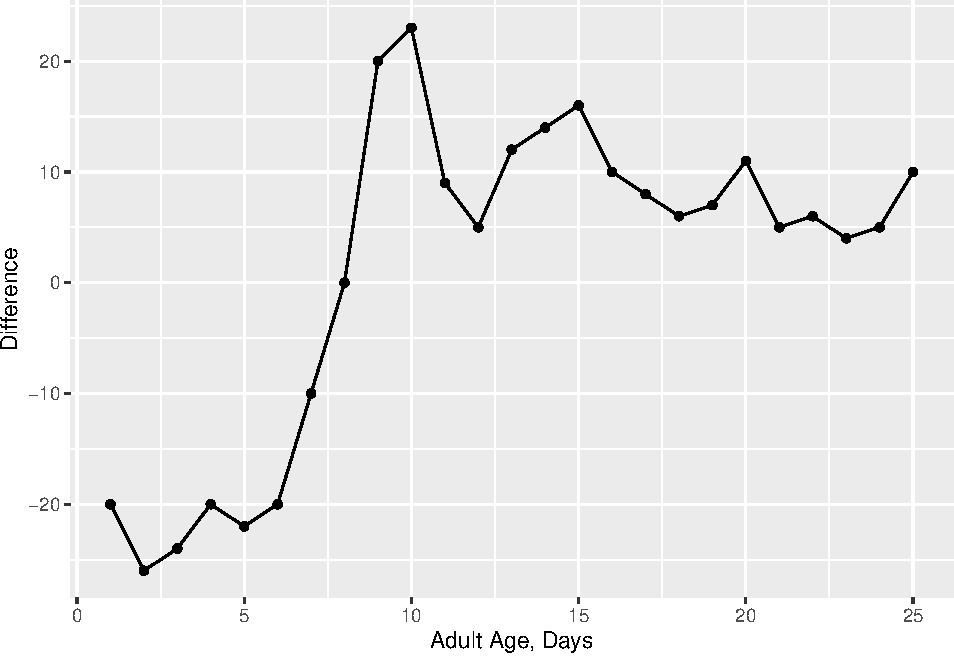
\includegraphics{BIOL-3295_files/figure-latex/unnamed-chunk-1-1.pdf}

\textbf{FIGURE 3.1} Difference in per capita egg production between the O lines and B lines from Rose and Charlesworth's (1981) experiment.

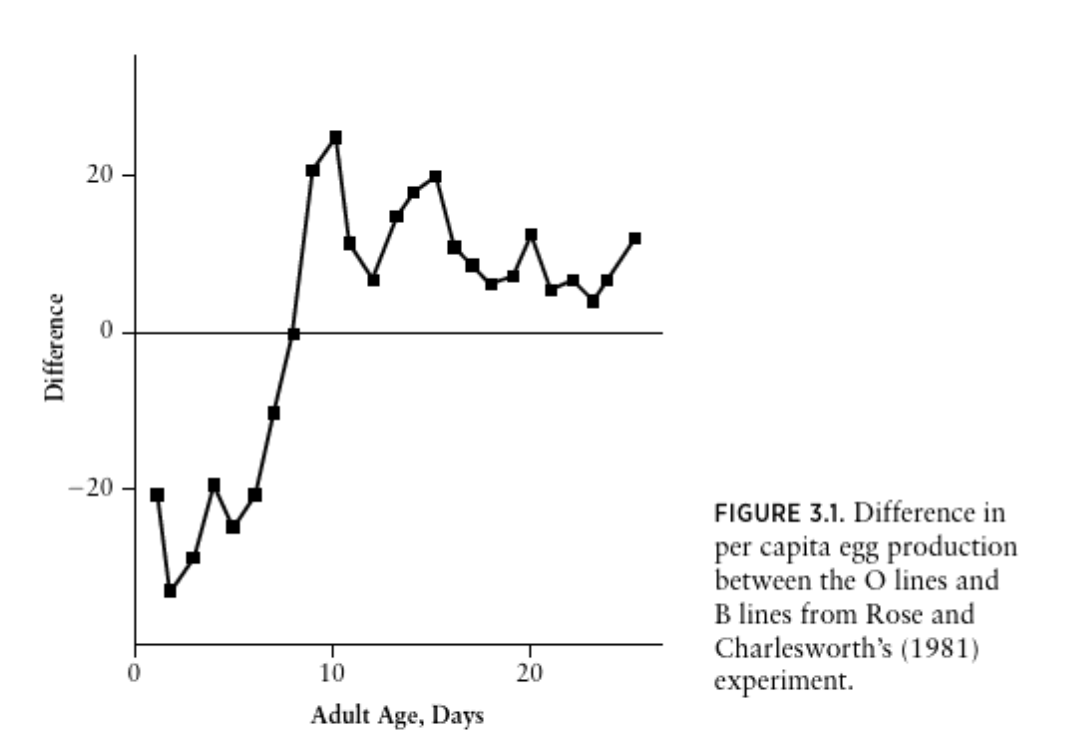
\includegraphics[width=0.9\linewidth]{figures/actual-fig}

\begin{center}\rule{0.5\linewidth}{0.5pt}\end{center}

Instructions to complete PART I are \protect\hyperlink{partI}{here}.

\textbf{PART II} of this assignment is to clean up messy data. As a biologist, much of my coding work involves getting data into the right format to use in functions, this might be a plot function like \texttt{ggplot()}, which you used in PART I, or a statistical function like \texttt{lm()}, which will perform a regression, t-test, or analysis of variance. The objective of PART II is to practice cleaning messy data into a useable format.

\begin{enumerate}
\def\labelenumi{\arabic{enumi}.}
\tightlist
\item
  You are to clean the messy data from \href{https://datacarpentry.org/semester-biology/exercises/Tidy-data-improving-messy-data-SQL/}{here} enough so you can make a plot using \texttt{ggplot()}. Some helpful instructions for how to do this are \protect\hyperlink{partII}{here}. The code that you write \textbf{must use the \texttt{select()}, \texttt{mutate()}, and \texttt{ggplot()} functions}. The graph that you make must be different than the example given in the instructions - for example, you might plot the same variables but for Plot 2.
\end{enumerate}

(perhaps this sounds easy - this data is pretty messy - I found it quite hard!)

\textbf{TO HAND IN}

\begin{enumerate}
\def\labelenumi{\arabic{enumi}.}
\tightlist
\item
  Hand in an \texttt{.Rmd} file and an output file (\texttt{.html}, \texttt{.docx}, or \texttt{.pdf}) with the solutions to both PART I and PART II of this assignment. Each part is 10 marks for a total of 20 marks.
\end{enumerate}

\hypertarget{jan-13-geometric-growth}{%
\chapter{Jan 13: Geometric growth}\label{jan-13-geometric-growth}}

\hypertarget{reading}{%
\section{Reading}\label{reading}}

Vandermeer, J.H., Goldberg, D.E., 2013. Population Ecology: First Principles (Second Edition). Princeton University Press, Princeton, United States. \textbf{p1-3.} \href{https://ebookcentral-proquest-com.qe2a-proxy.mun.ca/lib/mun/detail.action?docID=1205619}{Link}

\begin{itemize}
\item
  Von Foerster human population become effectively infinite on Nov 13 2026
\item
  Lilly pads replicate once per week. If it take a year for 1/2 a pond to be covered, when will it be completely covered? See also the \href{https://en.wikipedia.org/wiki/Wheat_and_chessboard_problem}{wheat and chessboard}
\item
  \(N_{t+1} = \lambda N_t\) equation 3 in \href{https://ebookcentral-proquest-com.qe2a-proxy.mun.ca/lib/mun/detail.action?docID=1205619}{Vandermeer and Goldberg}. For what values of \(\lambda\) will the population size, \(N_t\), grow?
\item
  \(N_t = N_0 \lambda^t\) is equation 4 in \href{https://ebookcentral-proquest-com.qe2a-proxy.mun.ca/lib/mun/detail.action?docID=1205619}{Vandermeer and Goldberg} (but written more generally). With \(N_0 > 0\) sketch a graph of \(N_t\) for different values of \(\lambda\). If \(N_0 = 0\), sketch a graph of \(N_t\).
\item
  If \(N_0 = 1.1\) individuals per km\(^2\), \(\lambda = 2\), what is is the population size at time \(t = 10\)?
\item
  Consider population growth of pheasants on \protect\hyperlink{pheasant}{Protection Island}. If we were to apply the geometric growth model to the pheasant population, what are some assumptions? How might this affect our parameterization (i.e., our estimate of \(\lambda\)) for the pheasant population?
\item
  How can we understand what \(\lambda\) is in a population that has births and deaths?
\end{itemize}

\hypertarget{pheasant}{%
\chapter{Jan 17: Geometric growth}\label{pheasant}}

\hypertarget{reading-1}{%
\section{Reading}\label{reading-1}}

Download the .pdf of the MSc thesis below and read the Abstract (the first two pages prior to the title page). Pay specific attention to the number of pheasants at different points in time, these might be \(N_{t+1}\) and \(N_t\) in the geometric growth model formula; and the number of births and deaths that occur, these may help you estimate \(\lambda\) in the geoemtric growth formula. Pay attention to the length of time that births and deaths are reported over, and what time of the year the population size is reported.

Newcomb, HR. 1940. \href{https://ir.library.oregonstate.edu/concern/graduate_thesis_or_dissertations/js956j801?locale=en}{Ring-necked pheasant studies on Protection Island in the Strait of Juan de Fuca}, Washington. MS thesis. Oregon State University. {[}two pages prior to the title page{]}

Noteably,

\begin{enumerate}
\def\labelenumi{\alph{enumi}.}
\tightlist
\item
  Pheasant chicks are born during the summer.
\item
  In May 1937, 10 pheasants were introduced to the island. Before the next breeding season there were 35.
\item
  November 10, 1938 a census estimated 110 pheasants.
\item
  October 13, 1939 a census estimated 400 pheasants.
\item
  Between the 1938 and 1939 censuses, Newcomb observed that 17 adult birds died.
\item
  During the 1938 nesting season there were 5.86 eggs/nest. 83.57\% of eggs hatched.
\item
  During the 1939 nesting season there were 8.73 eggs/nest. 64.58\% hatched.
\item
  During the 1939 nesting season: Average number of chicks per clutch was 6.93.\(^1\)
\item
  You can assume the sex ratio is 50:50 male to female. Pheasants are a sexually reproducing species.
\end{enumerate}

\(^1\) Note that g. and h. appear to be contradictory.

\hypertarget{questions}{%
\section{Questions}\label{questions}}

This approach is called independent parameter estimation because we will estimate the birth and mortality rates independently of the population size data for different years.

\begin{enumerate}
\def\labelenumi{\arabic{enumi}.}
\item
  \(b > 0\) is the per capita number of births each year. The estimation of \(b\) for a geometric growth model is more subtle. First, \(b\) is estimated as the number of births (occurring between \(t\) and \(t+1\)), divided by the number of individuals that could have given birth, \(N_t\). You might average this value across multiple years if sufficient data are available. Furthermore, to correctly project the future population size, we should consider what we have assumed about survival of the pheasant chicks, given the time step of our model. \textbf{Given a.-i. estimate \(b\). Write down any assumptions you have made.}
\item
  Is the probability that pheasants survive from one time step to the next. Estimate \(d\).
\item
  What is the value of \(\lambda\) given your estimate of \(b\) and \(d\) from previous questions? Is this population is expected to grow over time?
\item
  Lets assume that the pheasant population on Protection Island grows geometrically (i.e.~exponentially but for a discrete time model) where the geometric growth rate, \(\lambda\), is the value that you estimated in question 3. Let \(N_0 = 10\) and let \(t\) be the number of years since May 1937. Recall that when a population grows geometrically,
\end{enumerate}

\[ N_t = N_0 \lambda^t \]

Use the formula and your answer to 3. to predict the number of pheasants in May 1938, May 1939, May 1940, and May 1950.

\hypertarget{estimate}{%
\chapter{\texorpdfstring{Jan 19: \textbf{ASSIGNMENT} Estimating the geometric growth rate}{Jan 19: ASSIGNMENT Estimating the geometric growth rate}}\label{estimate}}

ASSIGNMENT 2 due Jan 26.

You are to write an Rmarkdown report that estimates the geometric growth rate, \(\lambda\), for the \protect\hyperlink{pheasant}{Protection Island pheasant population}. Your report needs to consider two methods for estimating the geometric growth rate: fitting; and estimation from independent data.

The code you will need to complete this assignment is below. You may copy and paste this code into your Rmarkdown report. Sometimes you will need to change the values.

The requirements of the report follow the code.

\hypertarget{code}{%
\section{Code}\label{code}}

\hypertarget{loading-and-plotting-the-data}{%
\subsection{Loading and plotting the data}\label{loading-and-plotting-the-data}}

Load the data. I copied the data on to a website, so it can be loaded with the command below. Click \href{https://github.com/ahurford/biol-4605-data/blob/main/data/protection-island.csv}{here} to view the code on the website.

\begin{Shaded}
\begin{Highlighting}[]
\NormalTok{data }\OtherTok{=} \FunctionTok{read.csv}\NormalTok{(}\StringTok{"https://raw.githubusercontent.com/ahurford/biol{-}4605{-}data/main/data/protection{-}island.csv"}\NormalTok{)}
\end{Highlighting}
\end{Shaded}

Let's plot the data. We select only columns 1 and 2 of the data because column 3 contains comments. We plot \texttt{year} on the horizontal (x-) axis and \texttt{size} on the (y-) vertical axis.

\begin{Shaded}
\begin{Highlighting}[]
\FunctionTok{require}\NormalTok{(ggplot2)}
\NormalTok{protection.island }\OtherTok{\textless{}{-}}\NormalTok{ data[,}\DecValTok{1}\SpecialCharTok{:}\DecValTok{2}\NormalTok{]}

\NormalTok{g1 }\OtherTok{=} \FunctionTok{ggplot}\NormalTok{(}\AttributeTok{data =}\NormalTok{ protection.island, }\FunctionTok{aes}\NormalTok{(}\AttributeTok{x =}\NormalTok{ year, }\AttributeTok{y =}\NormalTok{ size)) }\SpecialCharTok{+} 
  \FunctionTok{geom\_point}\NormalTok{() }\SpecialCharTok{+}
  \FunctionTok{xlab}\NormalTok{(}\StringTok{"year"}\NormalTok{)}\SpecialCharTok{+}
  \FunctionTok{ylab}\NormalTok{(}\StringTok{"population size"}\NormalTok{)}\SpecialCharTok{+}
  \FunctionTok{ggtitle}\NormalTok{(}\StringTok{"Protection Island"}\NormalTok{)}
\NormalTok{g1}
\end{Highlighting}
\end{Shaded}

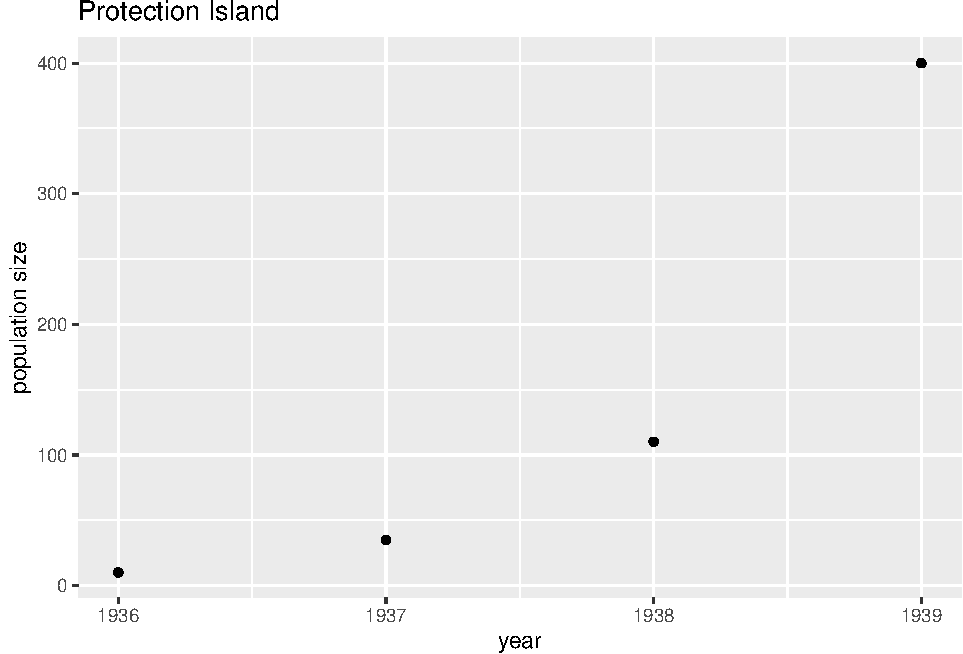
\includegraphics{BIOL-3295_files/figure-latex/unnamed-chunk-4-1.pdf}

\hypertarget{function-for-geometric-growth}{%
\subsection{Function for geometric growth}\label{function-for-geometric-growth}}

Below is the definition of a geometric growth function with time, \(t\), specifically defined for the number of years of Protection Island pheasant data, and the initial population size, \(N_0\), defined specifically for the Protection Island data. You need to give this function in your code \emph{before} you call the function.

\begin{Shaded}
\begin{Highlighting}[]
\NormalTok{geo.pred }\OtherTok{\textless{}{-}} \ControlFlowTok{function}\NormalTok{(lambda)\{}
\NormalTok{  t }\OtherTok{=}\NormalTok{ protection.island}\SpecialCharTok{$}\NormalTok{year }\SpecialCharTok{{-}}\NormalTok{ protection.island}\SpecialCharTok{$}\NormalTok{year[}\DecValTok{1}\NormalTok{]}
\NormalTok{  N0 }\OtherTok{=}\NormalTok{ protection.island}\SpecialCharTok{$}\NormalTok{size[}\DecValTok{1}\NormalTok{]}
\NormalTok{  size }\OtherTok{=}\NormalTok{ N0}\SpecialCharTok{*}\NormalTok{lambda}\SpecialCharTok{\^{}}\NormalTok{t}
\NormalTok{  pred }\OtherTok{=} \FunctionTok{data.frame}\NormalTok{(}\AttributeTok{year =}\NormalTok{ protection.island}\SpecialCharTok{$}\NormalTok{year, }\AttributeTok{size =}\NormalTok{ size)}
\NormalTok{\}}
\end{Highlighting}
\end{Shaded}

The function is called by running \texttt{geo.pred(lambda)} in the console, where you enter a specific value for \texttt{lambda}.

After you have run the code (i.e.~in the Console) that defines the \texttt{geo.pred(lambda)} function (above), try \texttt{lambda\ =\ 3} as:

\begin{Shaded}
\begin{Highlighting}[]
\NormalTok{result }\OtherTok{=} \FunctionTok{geo.pred}\NormalTok{(}\DecValTok{3}\NormalTok{)}
\NormalTok{result}
\end{Highlighting}
\end{Shaded}

\begin{verbatim}
##   year size
## 1 1936   10
## 2 1937   30
## 3 1938   90
## 4 1939  270
\end{verbatim}

\textbf{Question 1} The \texttt{geo.pred()} function works by running the lines of code inside the \texttt{geo.pred()} function definition for the value of \texttt{lambda} that you supply (inside the parentheses in the function call). In the function definition, what are the lines of code that are pasted below doing? (Hint: What is the data frame \texttt{protection.island}? Note that \texttt{data{[}1{]}} selects the first value of a list of values and the \texttt{\$} selects a particular column of a data frame).

\begin{Shaded}
\begin{Highlighting}[]
\NormalTok{  t }\OtherTok{=}\NormalTok{ protection.island}\SpecialCharTok{$}\NormalTok{year }\SpecialCharTok{{-}}\NormalTok{ protection.island}\SpecialCharTok{$}\NormalTok{year[}\DecValTok{1}\NormalTok{]}
\NormalTok{  N0 }\OtherTok{=}\NormalTok{ protection.island}\SpecialCharTok{$}\NormalTok{size[}\DecValTok{1}\NormalTok{]}
\end{Highlighting}
\end{Shaded}

\hypertarget{fitting-lambda}{%
\subsection{Fitting lambda}\label{fitting-lambda}}

We have defined a function that will predict the population size of pheasants on Protection Island for different user supplied values of \texttt{lambda}. But what value of \texttt{lambda} is most likely given the data?

To answer this question we will use a statistical method known as maximum likelihood.

Our first step is to define a function that quantifies the fit of a given \texttt{lambda} value. This function assumes that deviations of the recorded data from the model-predicted values follow a Poisson distribution:

\begin{Shaded}
\begin{Highlighting}[]
\NormalTok{geofit }\OtherTok{\textless{}{-}} \ControlFlowTok{function}\NormalTok{(lambda)\{}
\NormalTok{  pred}\OtherTok{=}\FunctionTok{geo.pred}\NormalTok{(}\AttributeTok{lambda=}\NormalTok{lambda)}
\NormalTok{  Ypred }\OtherTok{=}\NormalTok{ pred}\SpecialCharTok{$}\NormalTok{size}
  \SpecialCharTok{{-}}\FunctionTok{sum}\NormalTok{(}\FunctionTok{dpois}\NormalTok{(protection.island}\SpecialCharTok{$}\NormalTok{size, Ypred, }\AttributeTok{log=}\NormalTok{T))}
\NormalTok{\}}
\end{Highlighting}
\end{Shaded}

After running the \texttt{geo.fit(lambda)} function (in the Console), lets try to use the function and get some values of the negative log likelihood (i.e.~the fit):

\begin{Shaded}
\begin{Highlighting}[]
\FunctionTok{geofit}\NormalTok{(}\DecValTok{3}\NormalTok{)}
\end{Highlighting}
\end{Shaded}

\begin{verbatim}
## [1] 41.64846
\end{verbatim}

\begin{Shaded}
\begin{Highlighting}[]
\FunctionTok{geofit}\NormalTok{(}\DecValTok{1}\NormalTok{)}
\end{Highlighting}
\end{Shaded}

\begin{verbatim}
## [1] 1280.129
\end{verbatim}

This result tells us that given the data \texttt{lambda\ =\ 3} is much more likely than \texttt{lambda\ =\ 1} because the negative log likelihood value (41.65) is much smaller.

But what value of \texttt{lambda} is most likelihood given the data? i.e., for what value of \texttt{lambda} is the negative log likelihood minimized? To answer this question we need to call a function that will perform an optimization. This requires the \texttt{mle2} function from the \texttt{bbmle} package, and you will need to install this package prior to using this function.

\begin{Shaded}
\begin{Highlighting}[]
\FunctionTok{library}\NormalTok{(bbmle)}
\end{Highlighting}
\end{Shaded}

\begin{verbatim}
## Loading required package: stats4
\end{verbatim}

\begin{Shaded}
\begin{Highlighting}[]
\NormalTok{fit.geo }\OtherTok{\textless{}{-}} \FunctionTok{mle2}\NormalTok{(geofit, }\AttributeTok{start=}\FunctionTok{list}\NormalTok{(}\AttributeTok{lambda=}\DecValTok{3}\NormalTok{))}
\FunctionTok{summary}\NormalTok{(fit.geo)}
\end{Highlighting}
\end{Shaded}

\begin{verbatim}
## Maximum likelihood estimation
## 
## Call:
## mle2(minuslogl = geofit, start = list(lambda = 3))
## 
## Coefficients:
##        Estimate Std. Error z value     Pr(z)    
## lambda 3.408974   0.053472  63.752 < 2.2e-16 ***
## ---
## Signif. codes:  0 '***' 0.001 '**' 0.01 '*' 0.05 '.' 0.1 ' ' 1
## 
## -2 log L: 24.32396
\end{verbatim}

\begin{Shaded}
\begin{Highlighting}[]
\FunctionTok{confint}\NormalTok{(fit.geo)}
\end{Highlighting}
\end{Shaded}

\begin{verbatim}
##    2.5 %   97.5 % 
## 3.304256 3.513845
\end{verbatim}

The output above tells us that the maximum likelihood estimate of \texttt{lambda} is 3.41 and that the 95\% confidence interval is {[}3.30, 3.51{]}.

\hypertarget{plotting-the-fit}{%
\subsection{Plotting the fit}\label{plotting-the-fit}}

Finally, we would like to use our estimate values of \texttt{lambda} in the geometric growth function and compare the fitted values with the observed data.

In the code below, \texttt{lambda\ =\ 3} is the estimated lambda value, and the 95\% confidence interval is {[}2,4{]}. To use this code for your assignment you will need to substitute different values.

\begin{Shaded}
\begin{Highlighting}[]
\NormalTok{fit.predictions }\OtherTok{=} \FunctionTok{geo.pred}\NormalTok{(}\DecValTok{3}\NormalTok{)}\SpecialCharTok{$}\NormalTok{size}
\NormalTok{lower.fit }\OtherTok{=} \FunctionTok{geo.pred}\NormalTok{(}\DecValTok{2}\NormalTok{)}\SpecialCharTok{$}\NormalTok{size}
\NormalTok{upper.fit }\OtherTok{=} \FunctionTok{geo.pred}\NormalTok{(}\DecValTok{4}\NormalTok{)}\SpecialCharTok{$}\NormalTok{size}
\end{Highlighting}
\end{Shaded}

We had already made a plot of the data and we named our graph \texttt{g1}. We can now add some more layers to the graph as shown below. Note that the line is the value of \texttt{fit.predictions} as defined above (i.e., set \texttt{=3} as an example), and the shaded ribbon spans from \texttt{lower.fit} to \texttt{upper.fit} (i.e., set to \texttt{1} and \texttt{2} as an example).

\begin{Shaded}
\begin{Highlighting}[]
\NormalTok{g2 }\OtherTok{=}\NormalTok{ g1 }\SpecialCharTok{+}
  \FunctionTok{geom\_line}\NormalTok{(}\FunctionTok{aes}\NormalTok{(}\AttributeTok{y=}\NormalTok{fit.predictions)) }\SpecialCharTok{+}
  \FunctionTok{geom\_ribbon}\NormalTok{(}\FunctionTok{aes}\NormalTok{(}\AttributeTok{ymin =}\NormalTok{ lower.fit, }\AttributeTok{ymax =}\NormalTok{ upper.fit), }\AttributeTok{alpha =}\NormalTok{ .}\DecValTok{2}\NormalTok{)}
\NormalTok{g2}
\end{Highlighting}
\end{Shaded}

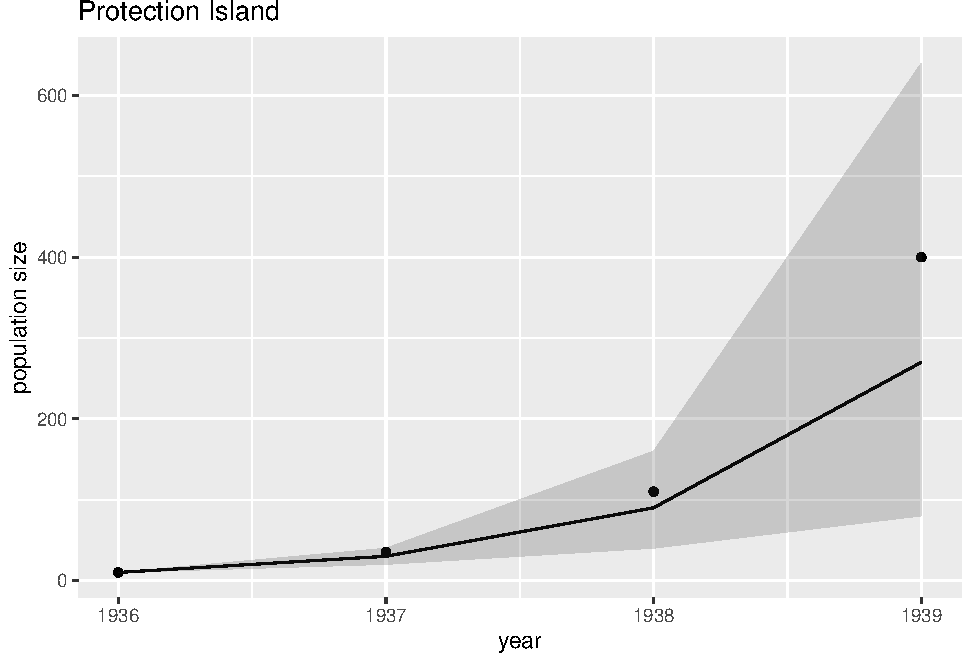
\includegraphics{BIOL-3295_files/figure-latex/unnamed-chunk-12-1.pdf}

\hypertarget{to-hand-in}{%
\section{To hand in}\label{to-hand-in}}

\begin{enumerate}
\def\labelenumi{\arabic{enumi}.}
\item
  Answer Question 1 which appears in bold in the \emph{Function for geometric growth} section.
\item
  Write an Rmarkdown report that estimates \(\lambda\) (i.e.~\texttt{lambda}) in the geometric growth rate function using maximum likelihood fitting.
  You must include a graph that shows:
\end{enumerate}

\begin{itemize}
\tightlist
\item
  The data (shown as dots);
\item
  The predicted values for the maximum likelihood estimate of \texttt{lambda} (shown as a line);
\item
  The predicted values for the 95\% confidence interval for the estimate of \texttt{lambda} (shown as a shaded region);
\end{itemize}

You must include a figure caption that explains the main point of your graph, and what the symbols are.

Your Rmarkdown file must contain a sequence of R commands that produces the graph.

\begin{enumerate}
\def\labelenumi{\arabic{enumi}.}
\setcounter{enumi}{2}
\tightlist
\item
  Estimate \(\lambda\) from data independent of the time series describing the population size of pheasants on Protection Island. This means that you cannot use more than one value of the population size to estimate one value of a quantity (you should be using the population size in a given year to calculate per capita rates by dividing only). You goal is to keep your parameter estimation method independent from the time series of pheasant population size so that you can \emph{validate} the assumptions of your geometric growth model. In your Rmarkdown report you should:
\end{enumerate}

\begin{itemize}
\item
  Derive a formula for \(\lambda\) in terms of \(b\) the per capita birth rate, and the probability of mortality \(d\) each year. Do this based on the class discussion on January 17 or by reading \href{https://ebookcentral.proquest.com/lib/mun/reader.action?docID=768551\&ppg=29}{Otto and Day, 2007} \emph{Section 2.5.1 Discrete-Time Models} p47-50 and omit migration, \(m=0\) for the application to the Protection Island pheasant population.
\item
  State some important assumptions of your \(\lambda\) formula.
\item
  Estimate \(b\) and \(d\) using some of the information given \protect\hyperlink{pheasant}{here}. Calculate \(\lambda\) given the formula you derived.
\item
  Use the \texttt{geo.pred(lambda)} function to predict the population size of pheasants on Protection Island for your independently estimated \(\lambda\) value. The code to do this must be included in your Rmarkdown file.
\item
  Make a plot of your predictions relative to the reported data. Include a figure caption that describes the main point of your figure and defines all the symbols.
\end{itemize}

\hypertarget{exponential}{%
\chapter{Jan 20: Exponential growth}\label{exponential}}

\hypertarget{required-reading}{%
\section{Required reading}\label{required-reading}}

Vandermeer, J.H., Goldberg, D.E., 2013. Population Ecology: First Principles (Second Edition). Princeton University Press, Princeton, United States. p4-8. \href{https://ebookcentral-proquest-com.qe2a-proxy.mun.ca/lib/mun/detail.action?docID=1205619}{Link}

We now have two ways of describing how population size changes with time whereby each individual has the same average number of offspring per unit time and the same probability of dying.

\begin{enumerate}
\def\labelenumi{\arabic{enumi})}
\tightlist
\item
  Discrete time geometric growth:
\end{enumerate}

\begin{equation}
N_t = N_0\lambda^t
\label{eq:Geo}
\end{equation}

and,

\begin{enumerate}
\def\labelenumi{\arabic{enumi})}
\setcounter{enumi}{1}
\tightlist
\item
  Continuous time exponential growth:
\end{enumerate}

\begin{equation}
N(t) = N(0)e^{rt}
\label{eq:Exp}
\end{equation}

Notably, for both these models the per capita birth and death rates do not change change over time, and do not change with density or age.

The notation \(N_t\) and \(N(t)\) is conventional for discrete time versus continuous time formulations respectively, however, these notations both mean the same: the population size at a particular time, \(t\). When \(t=0\) we have the population size at time 0: \(N_0\) or \(N(0)\).

As noted in the reading, when \(\lambda = e^{r}\) the equations are the same.

Note that \(e\) is the exponential function, \texttt{exp()} or \(e^x\).

\hypertarget{discrete-or-continuous-time-formulations}{%
\section{Discrete or continuous time formulations}\label{discrete-or-continuous-time-formulations}}

It is appropriate to use the discrete time formulation when births are synchronous.

It is appropriate to use the continuous time formulation when births occur throughout the year.

For example, for many animals there is a distinct breeding season: a short proportion of the year when offspring are born (synchronous reproduction). As such, there is very little temporal overlap between the times of year when births and deaths occur. Humans are an example of a species that might reasonably be modelled as continuous time because babies are born year round.

\hypertarget{questions-1}{%
\section{Questions}\label{questions-1}}

\begin{enumerate}
\def\labelenumi{\arabic{enumi}.}
\item
  For what values of \(r\) does the population size increase over time? Note that \(r\) might be negative, and I am asking not if the population size, \(N(t)\) is positive, but if the population is increasing, i.e., if \(N(t)\) is getting larger in value over time.
\item
  As described in the reading, \(b\) is a per capita birth rate, and \(d\) is a per capita death rate, and \(r = b-d\). For continuous time exponential growth, both \(b\) and \(d\) must be non-negative and can take any values bigger than 0. Note that this differs from the discrete time model formulation where \(0 \leq d \leq 1\). When \(d > 1\) in the continuous time formulation, this means that the average lifespan is less than one time step (i.e., the average life span is \(1/d\)). For example, when \(d = 2\) this means that the average life expectancy for an individual is 1/2 a time step (i.e., days or year, however, the time unit is defined in the model). When the population size increases over time, what is true of \(b\) relative to \(d\)?
\item
  For what value of \(r\) does \(N(t)\) not change over time? Hint: if \(N(t)\) is not changing then \(N(t)=N(0)\) for all \(t\).
\item
  Consider the equation:
  \[
  \frac{dN(t)}{dt} = rN(t).
  \]
  As described in the reading, this is an alternative way to write the continuous time exponential growth equation. The quantity \(\frac{dN(t)}{dt}\) can be understood as the slope of a graph where population size is on the vertical axis and time is on the horizontal axis. As such, if the slope is zero, \(\frac{dN(t)}{dt}=0\), then the population size is not changing. If \(\frac{dN(t)}{dt}<0\), then the population size is decreasing. For what value of \(r\) does the population size decrease? What is true about \(b\) relative to \(d\) in this instance?
\item
  Which population would be more appropriate to be modelled as a continuous time formulation: \emph{E. coli} bacteria or moose?
\item
  Calculate the formula for the doubling time for continuous time exponential growth (equation \eqref{eq:Exp}). This is the time for the population to double in size. The value of \(N(0)\), the population size at \(t=0\) doesn't matter as long as it is a positive number. When the population has doubled, \(N(t) = 2N(0)\). To answer this question you need to find \(t\) such that \(N(t) = 2N(0)\). You may need to revisit some rules about working with logarithms to complete this question (i.e.~see \href{https://en.wikipedia.org/wiki/Logarithm}{here}, specifically the \emph{Product, Quotient, Power, and Root} table.
\end{enumerate}

\hypertarget{dd}{%
\chapter{Jan 24: Density dependent growth}\label{dd}}

\hypertarget{required-reading-1}{%
\section{Required reading}\label{required-reading-1}}

Vandermeer, J.H., Goldberg, D.E., 2013. Population Ecology: First Principles (Second Edition). Princeton University Press, Princeton, United States. p9-17. \href{https://ebookcentral-proquest-com.qe2a-proxy.mun.ca/lib/mun/detail.action?docID=1205619}{Link}

\hypertarget{questions-2}{%
\section{Questions}\label{questions-2}}

\begin{enumerate}
\def\labelenumi{\arabic{enumi}.}
\item
  What is the equation for continuous time logistic growth in its \emph{classic form}? Define all the symbols in the equation by writing their meanings in words. Can \(K\) be negative?
\item
  What does dN/dt mean?
\item
  Assume that \(N < K\). For what values of \(r\) will \(N\) increase over time?
\item
  Assume that \(r > 0\) and \(K > N\). Will \(N\) increase or decrease in size over time?
\item
  Assume that \(r,K \neq 0\). For what values of \(N\) is the population size constant (i.e., not changing over time)?
\item
  What is the main difference between exponential and logistic growth?
\item
  Sketch a graph of the logistic growth equation, \(\frac{dN(t)}{dt} = rN(t)\left(1 - \frac{N(t)}{K}\right)\), with time, \(t\), on the horizontal axis (x-axis), and population size \(N(t)\), on the vertical (y-axis).
\end{enumerate}

\begin{enumerate}
\def\labelenumi{\alph{enumi}.}
\tightlist
\item
  Add to your graph a dashed line corresponding to the carrying capacity, \(N(t) = K\).
\item
  Label on your graph, \(N(0)\): the population size at \(t=0\).
\item
  As drawn in your graph, is \(N(0)<K\)? i.e.~is the population size at \(t=0\) less than the carrying capacity, \(K\)?
\item
  As drawn, is \(r > 0\)? i.e.~is the net reproductive rate when the population size is small, positive?
\item
  What does it mean if \(r<0\) in terms of the per capita birth rate when the population size is small, \(b\), relative to the per capita death rate when the population size is small, \(d\)?
\item
  If you answered `yes' to c.~add another line for \(N(t)\), but when \(N(0)>K\) (assume \(r>0\)). Note that \(N(0)>K\) means that at time \(t=0\) the population size, \(N(0)\), is greater than the carrying capacity, \(K\).
\end{enumerate}

\begin{enumerate}
\def\labelenumi{\arabic{enumi}.}
\item
  Draw a graph of a. exponential growth, \(N(t) = N(0)e^{rt}\) or \(\frac{dN(t)}{dt} = rN(t)\) (both are the same equation), and b. logistic growth \(\frac{dN(t)}{dt} = rN(t)\left(1 - \frac{N(t)}{K}\right)\), where the value of \(r\) is the same for both a. and b.
\item
  Draw a graph of logistic growth, where the population size is decreasing \(\frac{dN(t)}{dt}<0\), but positive \(N(t)>0\). Give a condition on the initial value of \(N(0)\) or the per capita net reproductive rate when the population size is small, \(r\), such that the population size is decreasing, \(\frac{dN(t)}{dt}<0\), but positive, \(N(t)>0\).
\end{enumerate}

\hypertarget{jan-26-density-dependence}{%
\chapter{Jan 26: Density dependence}\label{jan-26-density-dependence}}

I give the derivation of the logistic growth equation as from Vandermeer and Goldberg \href{https://www.youtube.com/watch?v=UisbkgNlaOE\&t=118s}{here}.

However, the logistic growth equation, in its classic form does not have a strong mechanistic basis making it difficult to parameterize.

These issues are discussed \href{https://www.sciencedirect.com/science/article/pii/S030438000400554X?via\%3Dihub}{here}

\hypertarget{jan-27-density-dependence-discrete-time}{%
\chapter{Jan 27: Density dependence (discrete time)}\label{jan-27-density-dependence-discrete-time}}

Density-yield and discrete time density dependence

\hypertarget{required-reading-2}{%
\section{Required reading}\label{required-reading-2}}

Vandermeer, J.H., Goldberg, D.E., 2013. Population Ecology: First Principles (Second Edition). Princeton University Press, Princeton, United States. p17-19 and 28-29. \href{https://ebookcentral-proquest-com.qe2a-proxy.mun.ca/lib/mun/detail.action?docID=1205619}{Link}

\hypertarget{questions-3}{%
\section{Questions}\label{questions-3}}

\begin{enumerate}
\def\labelenumi{\arabic{enumi}.}
\item
  Logistic growth assumes density dependence in the population growth rate. This, however, may be insufficient in many applications. In the section, \emph{The Yield-Density Relationship} what solution is proposed?
\item
  As written in Vandermeer and Goldberg the Shinozaki-Kira equation is presented without an \texttt{=}. Write the complete equation, by adding in an equals and quantity on the other size of the equals. Define all the parameters and variables in the equation.
\item
  The Beverton-Holt equation is equation (28) on p29. There are two values of \(N_t\) such that \(N_t = N_{t+1}\). One value can be found by re-arranging,
\end{enumerate}

\[
1 = \frac{\lambda}{1+\alpha N_t},
\]

until \(N_t\) is isolated on one side. To find the other value inspect the equation,

\[
N_{t+1} = \frac{\lambda N_t}{1+\alpha N_t}.
\]

What is another value of \(N_t\) such that \(N_{t+1}=N_t\).

\hypertarget{partI}{%
\chapter*{PART I - Instructions}\label{partI}}

For general instructions on installing \texttt{R}, \texttt{RStudio} and installing packages see the \href{https://ahurford.github.io/quant-guide-all-courses/}{Quantitative Training Manual}.

\begin{itemize}
\tightlist
\item
  \href{https://ahurford.github.io/quant-guide-all-courses/install.html}{Install} the \texttt{Rmarkdown} package and all dependencies.
\item
  Install \texttt{tinytex}. In the past we have had some problems with this on PCs. If your \texttt{tinytex} installation fails, what you might try is a package manager for Windows, i.e.~\texttt{Chocolatey} or \texttt{Scoop}. See \href{https://github.com/rstudio/tinytex-releases}{here} for details. You are unsuccessful at installing \texttt{tinytex} that is okay, this package is only necessary to produce a .pdf output. You can complete your assignment as a .docx output or .html output.
\end{itemize}

\textbf{Why use R markdown?}

\begin{itemize}
\item
  Integrate code and write-up to avoid mistakes moving between \texttt{.R} (or other software) for analysis and \texttt{.docx} for write-up.
\item
  It is easier to find all your work when everything is in one file (or linked to from one file).
\item
  Run code in the background of your write-up so that if something changes the write-up automatically updates in all the relevant places. The reduces the chances of errors in your write-up.
\item
  Publish your work as a website. This facilitates hyper-linking, you can update your work at any time, avoiding emailing your work keeps email storage free, and your work can be easily shared (i.e., in conversation I might say `that analysis is linked off my faculty website').
\item
  Include math symbols quickly because your hands don't leave the keyboard to make selections from drop-down menus.
\item
  If your analysis is time-consuming you might not want the calculations in your write-up, slowing the compilation of your write-up. In this case you might have a separate \texttt{.R} analysis file that outputs your results as a \texttt{.csv} or plot. You can read these in automatically to your write-up by specifying the path to the \texttt{.csv} or plot.
\end{itemize}

\begin{enumerate}
\def\labelenumi{\arabic{enumi}.}
\item
  In \texttt{R\ Studio}, select \texttt{File\ \textgreater{}\ New\ Project...\ \textgreater{}\ R\ Markdown}. Give the file a name, etc.
\item
  The default \texttt{.Rmd} opens already with some code to help you. With the default \texttt{.Rmd} opened, there should be a \texttt{Knit} button at the top and center of the Editor pane. Click the \texttt{Knit} button to knit to \texttt{.pdf}, \texttt{.html}, or \texttt{.docx} output. Alternatively, do \texttt{Cmd/Ctrl\ +\ Shift\ +\ K}.
\end{enumerate}

\begin{center}
\includegraphics[width=0.5\linewidth]{figures/Knit} \end{center}

\emph{(If this did not work, perhaps you have not installed the rmarkdown or tinytex packages)}

\begin{enumerate}
\def\labelenumi{\arabic{enumi}.}
\setcounter{enumi}{2}
\tightlist
\item
  Beside the \texttt{Knit} button is an arrow. You have the option to knit to \texttt{.pdf}, \texttt{.html}, or \texttt{.docx} output. Try producing other outputs.
\end{enumerate}

\emph{(For me, producing a .docx opened Skype (clearly a bug). This was fixed by using Finder (on my Mac) to find the .docx file that I made, and selecting Open With \textgreater{} Microsoft Word)}

\begin{enumerate}
\def\labelenumi{\arabic{enumi}.}
\setcounter{enumi}{3}
\tightlist
\item
  Below are some things to try, that will help you to complete PART I. Type the code, then \texttt{Knit} to see what happens.
\end{enumerate}

\begin{itemize}
\item
  Include variables in-text by enclosing in \texttt{\$x\$}, i.e.~this renders as \(x\), which is italicized to indicate in your writing that \(x\) is a variable rather than a letter.
\item
  \href{https://ahurford.github.io/quant-guide-all-courses/data-entry.html\#loading-or-importing-data}{Load data} using R commands. \emph{(If you want to do this quickly copy and paste the command at the end of this section)}
\item
  \href{https://bookdown.org/yihui/rmarkdown/r-code.html}{Hide the code} that loads the data in the output. i.e., read about the options for r code chunks: \texttt{echo}, \texttt{include}, \texttt{message}, \texttt{warning}, \texttt{eval}, and \texttt{results}. Print the data in your output. Show both the code and the output. Try it all!
\item
  Show only your code print out. Can you do this?
\end{itemize}

\begin{verbatim}
##   Psoil Pcorn
## 1     1    64
## 2     4    71
## 3     5    54
## 4     9    81
## 5    13    93
## 6    11    76
\end{verbatim}

\begin{itemize}
\item
  Include code in-text as \texttt{\textasciigrave{}r\ x\ \textasciigrave{}}. This renders as 80 because in a hidden coding block I loaded data and assigned \texttt{x\textless{}-mean(data\$Pcorn)}. Therefore, the reported value of \(x\) = 80 is the mean phosphorous in the soil for the data I loaded in the background. If the data change, the mean reported in this document will automatically change too.
\item
  Make \href{https://bookdown.org/yihui/rmarkdown/markdown-syntax.html\#block-level-elements}{headings, subheadings}, \href{https://bookdown.org/yihui/rmarkdown/markdown-syntax.html\#inline-formatting}{bold font}, etc.
\item
  Make a \href{https://bookdown.org/yihui/rmarkdown/markdown-syntax.html\#inline-formatting}{hyperlink}.
\item
  Use latex commands to include in-text equations, i.e., \texttt{\$y\ =\ \textbackslash{}beta\_0\ +\ \textbackslash{}beta\_1\ x\$} renders as \(y = \beta_0 + \beta_1 x\); \texttt{\$\textbackslash{}frac\{dy\}\{dt\}\ =\ e\^{}x\$} renders as \(\frac{dy}{dt} = e^x\). \emph{(You may need to type \texttt{require(tinytex)} in the Console to get this to work. `The website \href{https://detexify.kirelabs.org/classify.html}{Detexify} is fun for identifying latex commands for different symbols (Some advanced symbols may require packages that you haven't installed and therfore won't work))}.
\item
  Try some \href{https://bookdown.org/yihui/rmarkdown/markdown-syntax.html\#math-expressions}{more complicated} Latex.
\end{itemize}

\begin{Shaded}
\begin{Highlighting}[]
\NormalTok{data }\OtherTok{\textless{}{-}} \FunctionTok{read.csv}\NormalTok{(}\StringTok{\textquotesingle{}https://raw.githubusercontent.com/ahurford/biol{-}4605{-}data/main/data/corn.csv\textquotesingle{}}\NormalTok{, }\AttributeTok{fill=}\ConstantTok{TRUE}\NormalTok{)}
\end{Highlighting}
\end{Shaded}

\begin{itemize}
\item
  If you would like a more structured introduction to R Markdown you can read \href{https://bookdown.org/yihui/rmarkdown/}{R Markdown: the definitive guide}.
\item
  This \href{https://www.rstudio.com/wp-content/uploads/2015/02/rmarkdown-cheatsheet.pdf}{R markdown cheat sheet} is helpful.
\item
  Some more advanced skills you might learn are making alert boxes, or changing some of the options in the \href{https://bookdown.org/yihui/rmarkdown/html-document.html}{YAML}. The alert boxes in this document are made as \texttt{div\ class="alert\ alert-info"} between \texttt{\textless{}\ \textgreater{}}, then the text, and closed with \texttt{/div} between \texttt{\textless{}\ \textgreater{}}.
\item
  My experience making tables in \texttt{.Rmd} has not been good. Usually, I make the table in \texttt{.docx}, print to \texttt{.pdf}, take a screenshot and import the \texttt{.png} to \texttt{.Rmd} or \texttt{.tex}.
\end{itemize}

\begin{enumerate}
\def\labelenumi{\arabic{enumi}.}
\setcounter{enumi}{4}
\tightlist
\item
  For your PART I specifically, you need to make a figure in \texttt{ggplot}. For \texttt{ggplot} you need your data as a data frame. The code that I used in the example was:
\end{enumerate}

\begin{Shaded}
\begin{Highlighting}[]
\NormalTok{age }\OtherTok{=} \FunctionTok{seq}\NormalTok{(}\DecValTok{1}\NormalTok{,}\DecValTok{25}\NormalTok{)}
\NormalTok{difference }\OtherTok{=} \FunctionTok{c}\NormalTok{(}\SpecialCharTok{{-}}\DecValTok{20}\NormalTok{, }\SpecialCharTok{{-}}\DecValTok{26}\NormalTok{, }\SpecialCharTok{{-}}\DecValTok{24}\NormalTok{, }\SpecialCharTok{{-}}\DecValTok{20}\NormalTok{, }\SpecialCharTok{{-}}\DecValTok{22}\NormalTok{, }\SpecialCharTok{{-}}\DecValTok{20}\NormalTok{, }\SpecialCharTok{{-}}\DecValTok{10}\NormalTok{, }\DecValTok{0}\NormalTok{,}
               \DecValTok{20}\NormalTok{, }\DecValTok{23}\NormalTok{, }\DecValTok{9}\NormalTok{, }\DecValTok{5}\NormalTok{, }\DecValTok{12}\NormalTok{, }\DecValTok{14}\NormalTok{, }\DecValTok{16}\NormalTok{, }\DecValTok{10}\NormalTok{, }\DecValTok{8}\NormalTok{, }\DecValTok{6}\NormalTok{, }\DecValTok{7}\NormalTok{, }\DecValTok{11}\NormalTok{, }\DecValTok{5}\NormalTok{, }\DecValTok{6}\NormalTok{, }\DecValTok{4}\NormalTok{, }\DecValTok{5}\NormalTok{, }\DecValTok{10}\NormalTok{)}
\NormalTok{data }\OtherTok{=} \FunctionTok{data.frame}\NormalTok{(}\AttributeTok{age=}\NormalTok{age, }\AttributeTok{difference =}\NormalTok{ difference)}
\end{Highlighting}
\end{Shaded}

As you can see, I have guessed the values in the plot and entered them manually. This is okay for the purposes of completing your assignment. (Extra for experts - try a package like \href{https://github.com/adamkucharski/scrapR}{\texttt{scrapR}} or \href{https://github.com/tpoisot/digitize}{\texttt{digitize}}).

\begin{enumerate}
\def\labelenumi{\arabic{enumi}.}
\setcounter{enumi}{5}
\tightlist
\item
  You need to install \texttt{ggplot2}. You also need to load that package because we are going to use functions from it now (do this as \texttt{require(ggplot2)}). The code that I used to make my \texttt{ggplot} was:
\end{enumerate}

\begin{Shaded}
\begin{Highlighting}[]
\NormalTok{g1}\OtherTok{=}\FunctionTok{ggplot}\NormalTok{(}\AttributeTok{data =}\NormalTok{ data, }\FunctionTok{aes}\NormalTok{(}\AttributeTok{x =}\NormalTok{ age, }\AttributeTok{y =}\NormalTok{ difference)) }\SpecialCharTok{+} 
  \FunctionTok{geom\_point}\NormalTok{() }\SpecialCharTok{+}
  \FunctionTok{geom\_line}\NormalTok{() }\SpecialCharTok{+}
  \FunctionTok{xlab}\NormalTok{(}\StringTok{"Adult Age, Days"}\NormalTok{)}\SpecialCharTok{+}
  \FunctionTok{ylab}\NormalTok{(}\StringTok{"Difference"}\NormalTok{)}
\NormalTok{g1}
\end{Highlighting}
\end{Shaded}

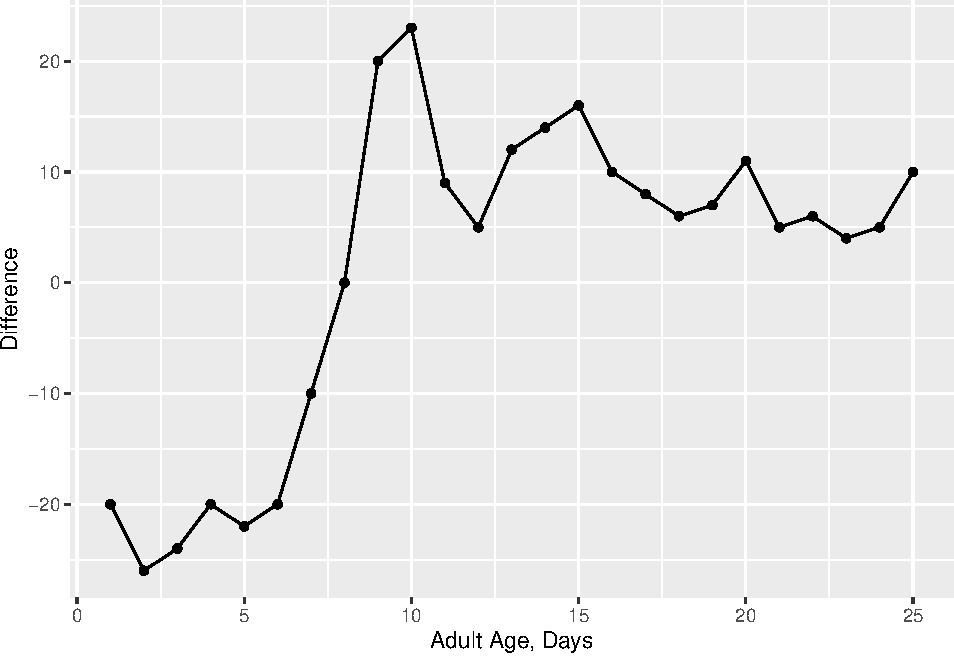
\includegraphics{BIOL-3295_files/figure-latex/unnamed-chunk-18-1.pdf}

If you need to add a title, you can add a layer \texttt{+\ ggtitle("Your\ title)}, to control the axis limits, use \texttt{+\ xlim(c(-10,10))} (with the values you need). Generally, you should be able to use an internet search to find what you need. You can also read more about \texttt{ggplot} \href{https://ahurford.github.io/quant-guide-all-courses/ggplot.html}{here}.

\begin{enumerate}
\def\labelenumi{\arabic{enumi}.}
\setcounter{enumi}{6}
\item
  To make your figure caption, just type below where your figure prints. To get bold text, use ** bold text ** (but without space between the ** and the text).
\item
  The last thing we need is to take a screenshot of the figure you are trying to reproduce, and to include it as a figure. I like to put all my figures in a folder named figure. You can read about including a \href{https://bookdown.org/yihui/rmarkdown/r-code.html\#figures}{figure} that is a \texttt{.png} or other format. Of the options, I find using knitr::include\_graphics() within a code chunk best because it seems easier to control the figure size. The code that I used in my example of how I completed PART I was:
\end{enumerate}

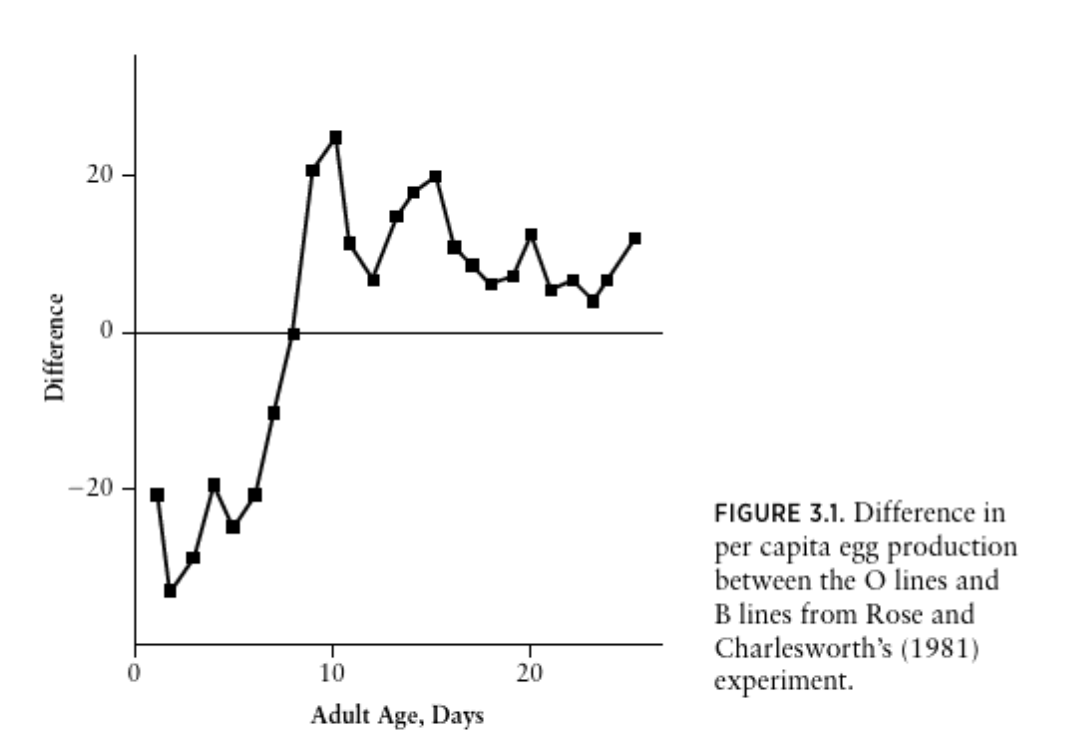
\includegraphics[width=0.9\linewidth]{figures/actual-fig}

Now you have all the information you need to complete PART I, you just need to put the pieces together. If you are stuck, ask me or a classmate.

\hypertarget{partII}{%
\chapter*{PART II - Instructions}\label{partII}}

\begin{itemize}
\item
  \href{https://ahurford.github.io/quant-guide-all-courses/install.html}{Install} the \texttt{dplyr} package, all dependencies, and load the package.
\item
  For instructions to clean data using tidyverse see \href{https://ahurford.github.io/quant-guide-all-courses/handling-data.html\#dplyr}{here}
\end{itemize}

First you need to \href{https://ahurford.github.io/quant-guide-all-courses/data-entry.html\#loading-or-importing-data}{load} the messy data from \href{https://datacarpentry.org/semester-biology/exercises/Tidy-data-improving-messy-data-SQL/}{here}.

It may be helpful to view the data in Excel to understand what it looks like before you import it to \texttt{R}.

Use \texttt{head(data)} in the Console, or \texttt{data} to view your data (where \texttt{data} is the name I gave my data).

\begin{Shaded}
\begin{Highlighting}[]
\FunctionTok{head}\NormalTok{(data)}
\end{Highlighting}
\end{Shaded}

\begin{verbatim}
##                 X          X.1       X.2      X.3    X.4 X.5            X.6
## 1                                                         NA               
## 2 Data for Site 7                                         NA               
## 3                                                         NA               
## 4         Plot: 1                                         NA        Plot: 2
## 5  Date collected       Family     Genus  Species Weight  NA Date collected
## 6        01/09/14 Heteromyidae Dipodomys merriami     40  NA       01/08/14
##          X.7     X.8      X.9   X.10 X.11           X.12             X.13
## 1                                      NA                                
## 2                                      NA                                
## 3                                      NA                                
## 4                                      NA        Plot: 3                 
## 5     Family   Genus  Species Weight   NA Date collected          Species
## 6 Cricetidae Neotoma albigula   -999   NA            1/8 Dipodomys ordii*
##     X.14
## 1       
## 2       
## 3       
## 4       
## 5 Weight
## 6     42
\end{verbatim}

These data are very messy indeed! A helpful command is to know the column names:

\begin{Shaded}
\begin{Highlighting}[]
\FunctionTok{colnames}\NormalTok{(data)}
\end{Highlighting}
\end{Shaded}

\begin{verbatim}
##  [1] "X"    "X.1"  "X.2"  "X.3"  "X.4"  "X.5"  "X.6"  "X.7"  "X.8"  "X.9" 
## [11] "X.10" "X.11" "X.12" "X.13" "X.14"
\end{verbatim}

\begin{Shaded}
\begin{Highlighting}[]
\CommentTok{\# Extract a row using tidyverse commands}
\NormalTok{dataX }\OtherTok{=}\FunctionTok{select}\NormalTok{(data, }\StringTok{"X"}\NormalTok{)}
\CommentTok{\# This is base R syntax to extract specifically rows 6 to 14}
\NormalTok{date.collected }\OtherTok{=}\NormalTok{ dataX}\SpecialCharTok{$}\NormalTok{X[}\DecValTok{6}\SpecialCharTok{:}\DecValTok{14}\NormalTok{]}
\CommentTok{\# as.Date() is needed for R to treat this variable as a date}
\NormalTok{date.collected }\OtherTok{=} \FunctionTok{as.Date}\NormalTok{(date.collected, }\AttributeTok{format =} \StringTok{"\%m/\%d/\%y"}\NormalTok{)}
\CommentTok{\# This prints to the output, so you can see what I have done}
\NormalTok{date.collected}
\end{Highlighting}
\end{Shaded}

\begin{verbatim}
## [1] "2014-01-09" "2014-01-09" "2014-01-09" "2014-01-09" "2014-01-20"
## [6] "2014-01-20" "2014-03-13" "2014-03-13" "2014-03-13"
\end{verbatim}

I will aim to make a data frame with ``date collected'' and ``weight'' for Plot 1. Inspecting the data, weight is \texttt{"X.4"} for Plot 1.

\begin{Shaded}
\begin{Highlighting}[]
\NormalTok{weight }\OtherTok{=} \FunctionTok{select}\NormalTok{(data, }\StringTok{"X.4"}\NormalTok{)}
\CommentTok{\# as.numeric() is needed because otherwise R doesn\textquotesingle{}t recognize these data as numbers {-} which I need for the multiplication later}
\NormalTok{weight }\OtherTok{=} \FunctionTok{as.numeric}\NormalTok{(weight}\SpecialCharTok{$}\NormalTok{X}\FloatTok{.4}\NormalTok{[}\DecValTok{6}\SpecialCharTok{:}\DecValTok{14}\NormalTok{])}
\CommentTok{\# Make this into a data frame so I can plot using ggplot}
\NormalTok{cleaned.data }\OtherTok{=} \FunctionTok{data.frame}\NormalTok{(date.collected, weight)}
\CommentTok{\# add a column that is a mutated column}
\NormalTok{cleaned.data }\OtherTok{=} \FunctionTok{mutate}\NormalTok{(cleaned.data,}\AttributeTok{weight.kg =}\NormalTok{ weight}\SpecialCharTok{/}\DecValTok{1000}\NormalTok{)}
\CommentTok{\# print the cleaned data so we can see what it looks like}
\NormalTok{cleaned.data}
\end{Highlighting}
\end{Shaded}

\begin{verbatim}
##   date.collected weight weight.kg
## 1     2014-01-09     40     0.040
## 2     2014-01-09     36     0.036
## 3     2014-01-09    135     0.135
## 4     2014-01-09     39     0.039
## 5     2014-01-20     43     0.043
## 6     2014-01-20    144     0.144
## 7     2014-03-13     51     0.051
## 8     2014-03-13     44     0.044
## 9     2014-03-13    146     0.146
\end{verbatim}

Now the data is in a format that I can make a plot:

\begin{Shaded}
\begin{Highlighting}[]
\FunctionTok{require}\NormalTok{(ggplot2)}
\NormalTok{g1}\OtherTok{=}\FunctionTok{ggplot}\NormalTok{(}\AttributeTok{data =}\NormalTok{ cleaned.data, }\FunctionTok{aes}\NormalTok{(}\AttributeTok{x =}\NormalTok{ date.collected, }\AttributeTok{y =}\NormalTok{ weight.kg)) }\SpecialCharTok{+} 
  \FunctionTok{geom\_point}\NormalTok{() }\SpecialCharTok{+}
  \FunctionTok{geom\_line}\NormalTok{() }\SpecialCharTok{+}
  \FunctionTok{xlab}\NormalTok{(}\StringTok{"Date collected"}\NormalTok{)}\SpecialCharTok{+}
  \FunctionTok{ylab}\NormalTok{(}\StringTok{"Weight in kg"}\NormalTok{)}
\NormalTok{g1}
\end{Highlighting}
\end{Shaded}

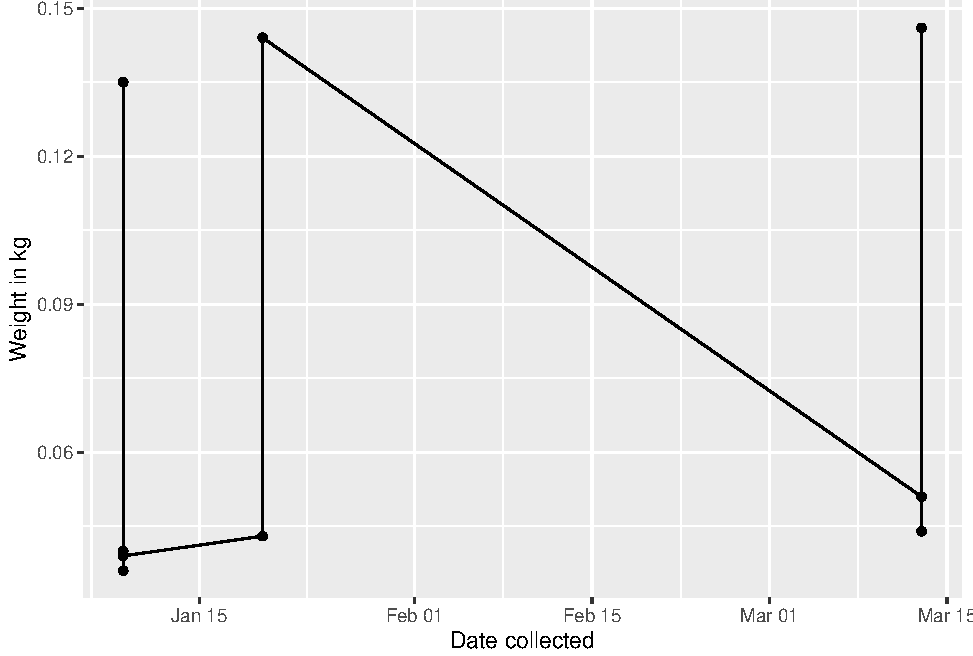
\includegraphics{BIOL-3295_files/figure-latex/unnamed-chunk-24-1.pdf}

\end{document}
